\documentclass[]{report}   
\usepackage{graphicx}

% type user-defined commands here

\begin{document}

\title{A demonstration of MRIVIEW}
\author{Dave Mattie}
\date{July 30, 2020}
\maketitle

I'm cheating a bit here buy not sourcing my example data from the internet.  Nifti files are big, and I have to send to the moon and back to get it (satellite internet).

This is a collage of different levels of a T1 Structural MRI

\begin{figure}[h!]
\centering
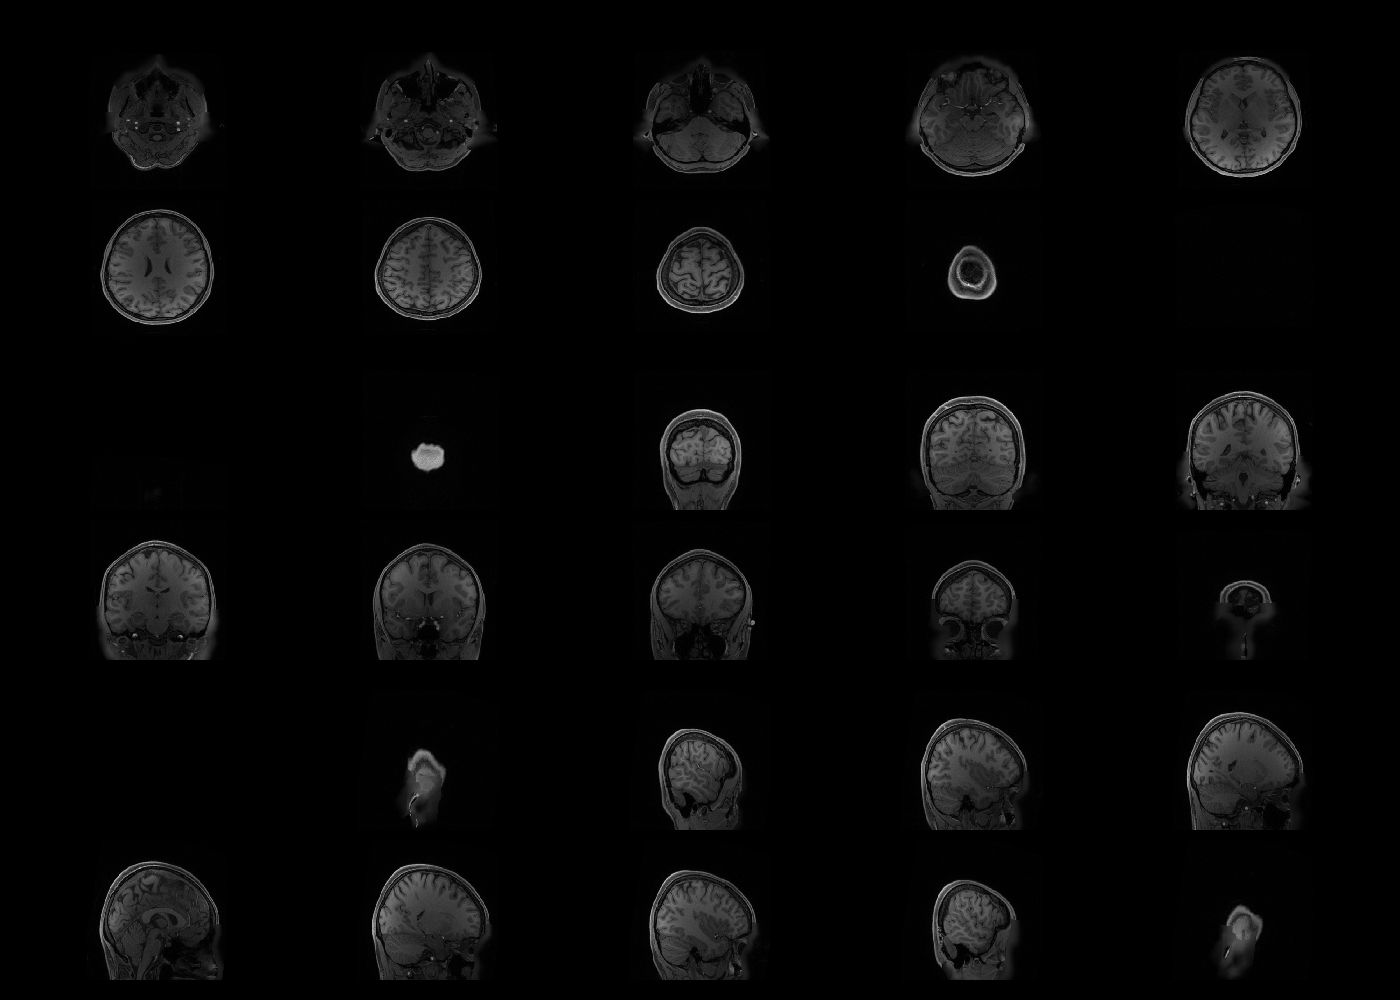
\includegraphics[scale=0.22]{collage}
\caption{Collage of different layers of MRI}
\label{fig:collage}
\end{figure}

This is a "carpet" to condense and represent a high density 4D nifti file

\begin{figure}[h!]
\centering
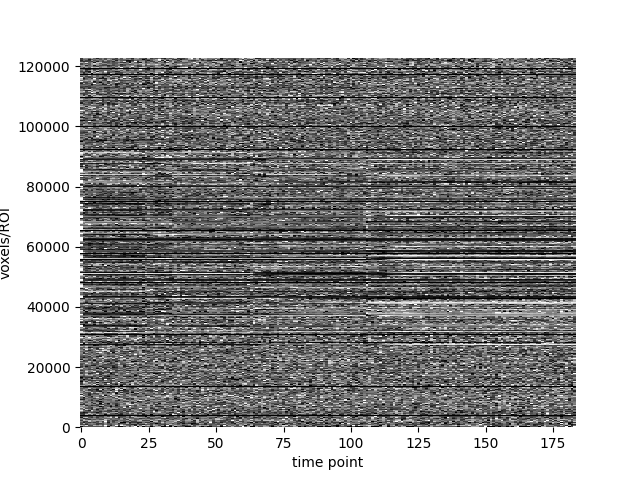
\includegraphics[scale=0.6]{carpet}
\caption{Carpet of 4D MRI}
\label{fig:carpet}
\end{figure}

\end{document}